\def\retinanet{
    RetinaNet\index{RetinaNet} \cite{lin2017focal} là một mô hình nhận diện đối tượng\index{nhận diện đối tượng} một pha\index{một pha} cân bằng giữa độ chính xác của các mô hình hai pha\index{hai pha} và tốc độ của các mô hình một pha\index{một pha} ở thời điểm đó.
    Nhóm tác giả của RetinaNet\index{RetinaNet} đưa ra vấn đề về các mô hình một pha\index{một pha} như YOLO \cite{redmon2016look} hay SSD \cite{liu2016ssd} dù đạt tốc độ rất nhanh nhưng lại kém các mô hình hai pha\index{hai pha} một khoảng rất xa về độ chính xác và đề xuất giải pháp khắc phục vấn đề này.

    \subsubsection*{Tổng quan các mô hình nhận diện đối tượng một pha}
    Các mô hình nhận diện đối tượng\index{nhận diện đối tượng} một pha\index{một pha} ở thời điểm đó đa phần đều chỉ sử dụng một mô hình xương sống CNN kết hợp thêm với các lớp Conv\index{lớp Conv} và lớp fully connected\index{lớp fully connected} để đưa ra dự đoán về lớp của đối tượng trong ảnh và độ lệch của hộp giới hạn\index{hộp giới hạn} so với groundtruth\index{groundtruth}.
    
    \begin{figure}[H]
        \centering
        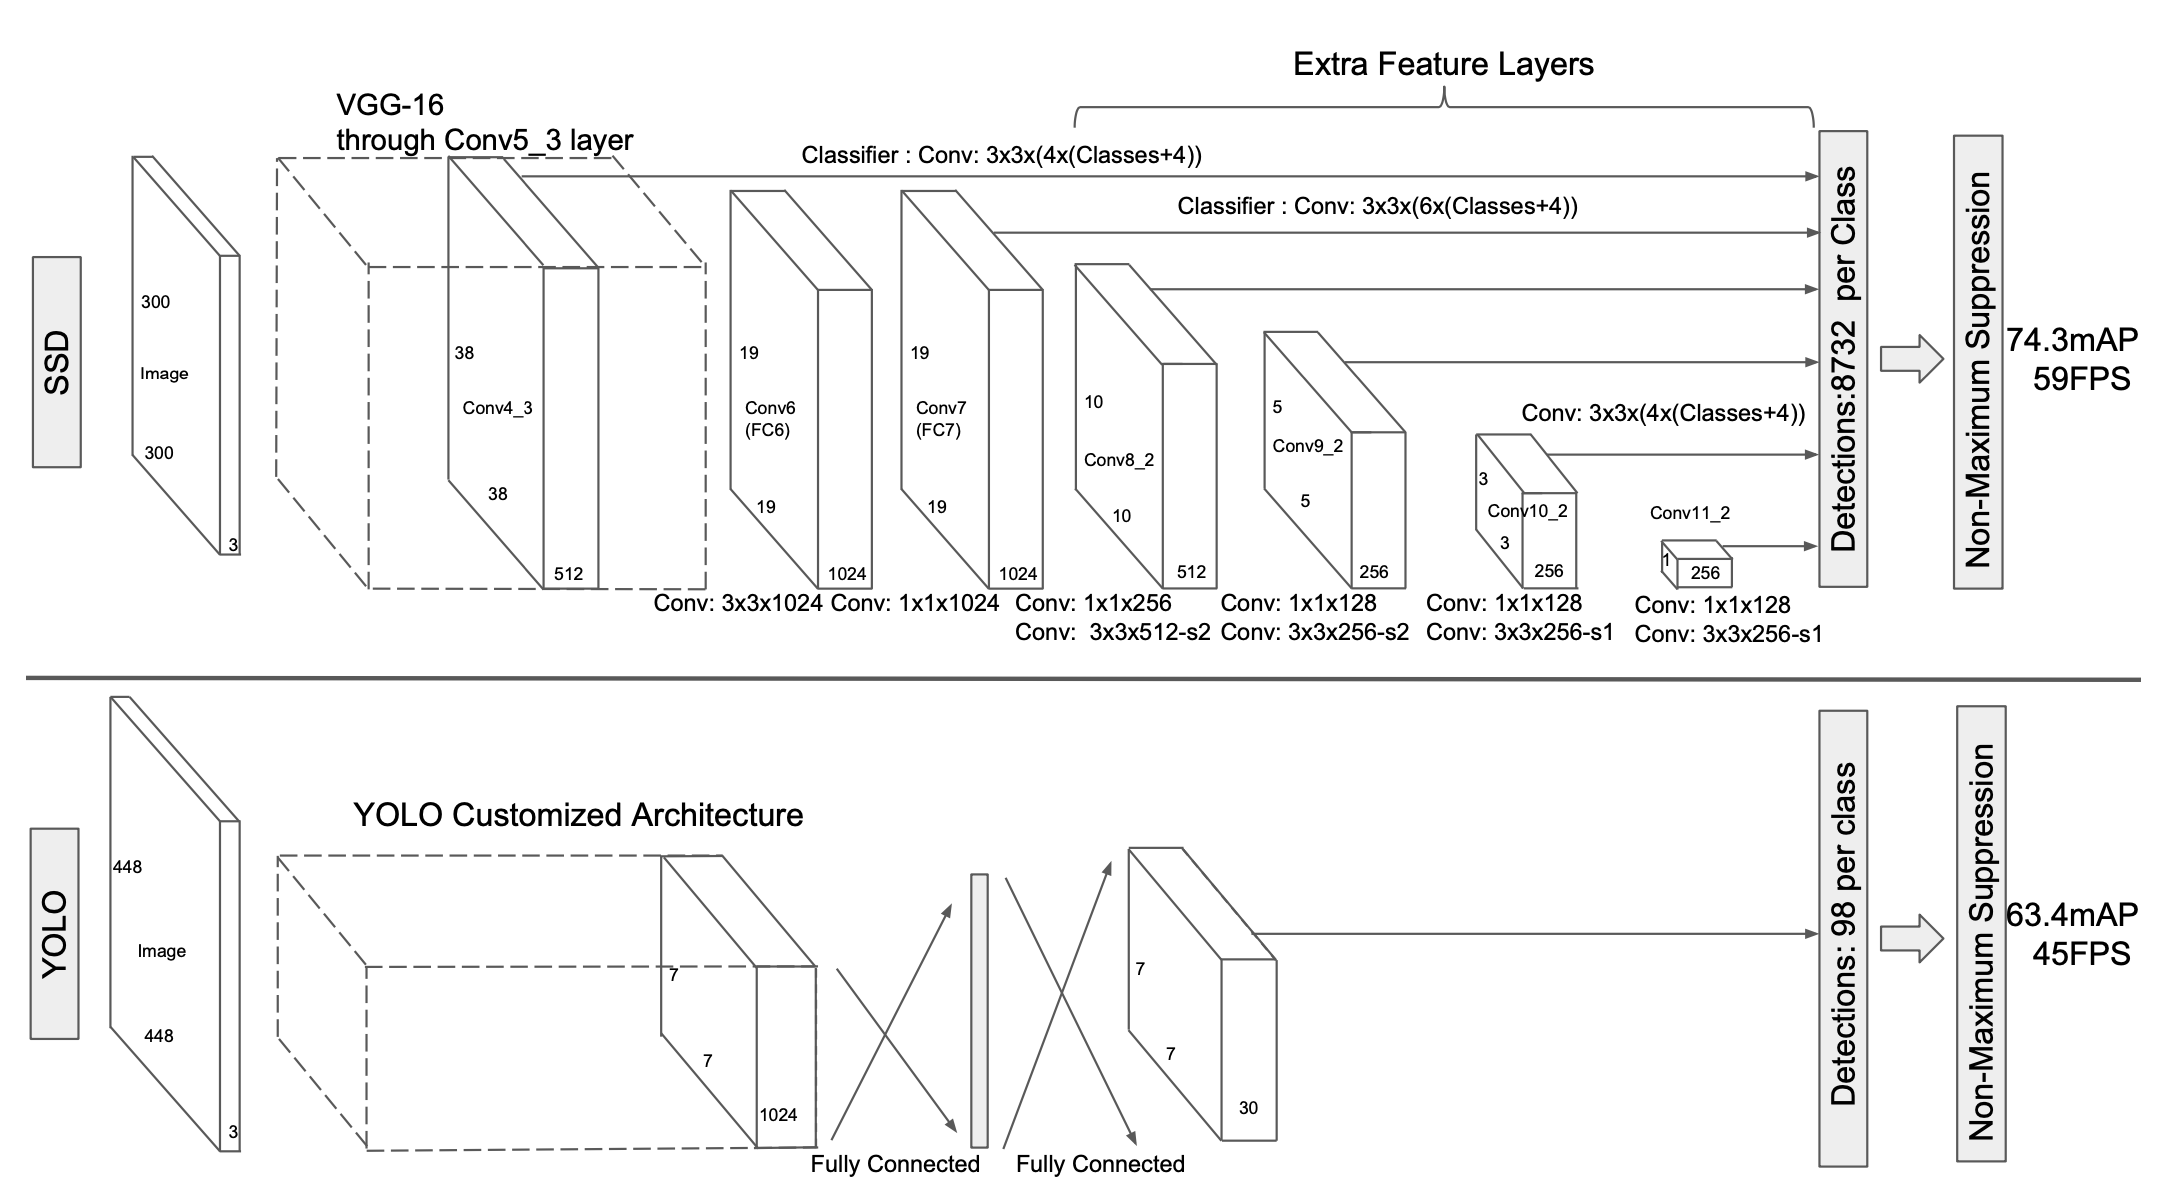
\includegraphics[width=14cm] {images/yolo_ssd_model}
        \caption{Chi tiết hai kiến trúc mô hình một pha\index{một pha} nổi tiếng là SSD và YOLO. (Nguồn: \cite{liu2016ssd})}
        \label{fig:yolo_ssd_model}
    \end{figure}

    \noindent
    Các mô hình nhận diện đối tượng\index{nhận diện đối tượng} một pha\index{một pha} cần phải xây dựng một phương pháp riêng nhằm đề xuất ra các khu vực mỏ neo\index{khu vực mỏ neo} chứa đối tượng.
    Hai mô hình nhận diện đối tượng\index{nhận diện đối tượng} một pha\index{một pha} nổi tiếng vào thời điểm đó là YOLO \cite{redmon2016look} và SSD \cite{liu2016ssd} có các cách đề xuất ra khu vực mỏ neo\index{khu vực mỏ neo} tương tự với nhau.
    
    \begin{figure}[H]
        \centering
        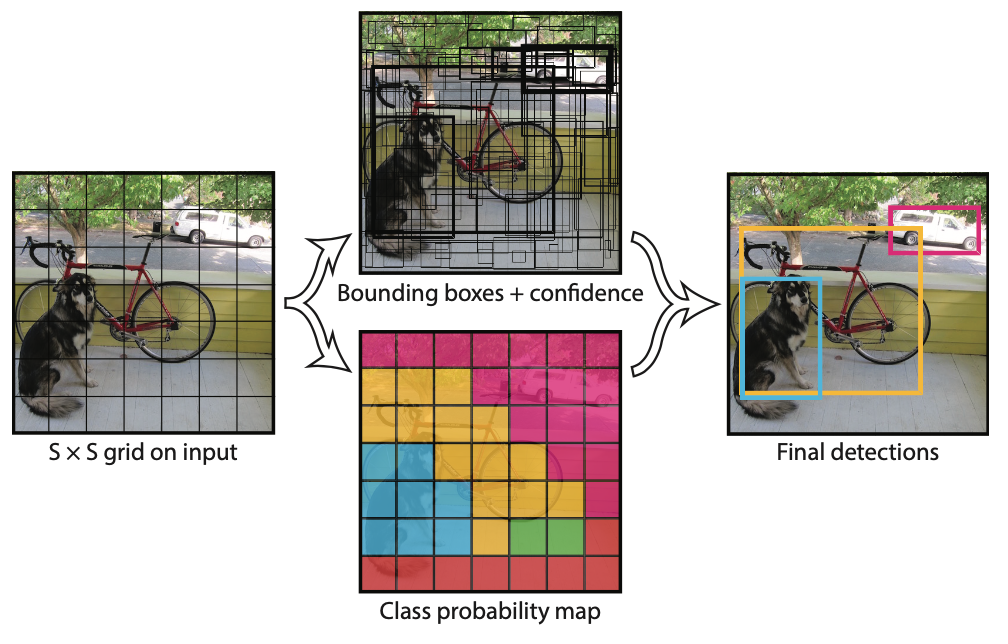
\includegraphics[width=11cm] {images/yolo_anchor}
        \caption{Cách đề xuất khu vực mỏ neo\index{khu vực mỏ neo} của mô hình YOLO. (Nguồn: \cite{redmon2016look})}
        \label{fig:yolo_anchor}
    \end{figure}

    \noindent
    YOLO đề xuất ra các khu vực mỏ neo\index{khu vực mỏ neo} thông qua việc chia ảnh đầu vào thành dạng grid\index{grid} có kích thước S x S và với mỗi grid\index{grid} sẽ trả đầu ra dự đoán có kích thước S x S x (B x 5 + C).
    Nếu tâm của một hộp giới hạn\index{hộp giới hạn} nằm trong ô nào trên grid\index{grid}, ô đó sẽ cần phải được dự đoán là chứa đối tượng.
    Mỗi ô trên grid\index{grid} sẽ được mô hình dự đoán (B x 5 + C) giá trị, trong đó: \\
    - B là số lượng hộp giới hạn\index{hộp giới hạn} dự đoán. \\
    - 5 là các giá trị trong đó có 4 giá trị x, y, w, h đại diện cho hộp giới hạn\index{hộp giới hạn} được dự đoán và 1 giá trị độ tự tin\index{độ tự tin}.
    Thay vì được học là 1 nếu khu vực mỏ neo\index{khu vực mỏ neo} có IoU\index{IoU} cao với groundtruth\index{groundtruth} hộp giới hạn\index{hộp giới hạn} và ngược lại là 0 nếu khu vực mỏ neo\index{khu vực mỏ neo} có IoU\index{IoU} thấp với groundtruth\index{groundtruth} hộp giới hạn\index{hộp giới hạn}, điểm đặc biệt về giá trị độ tự tin\index{độ tự tin} mà nhóm tác giả thiết kế trong mô hình YOLO là nó bằng chính giá trị IoU\index{IoU} so với groundtruth\index{groundtruth}. \\
    - C là số lượng lớp đối tượng\index{lớp đối tượng} trong bài toán nhận diện đối tượng\index{nhận diện đối tượng}.
    Mỗi giá trị dự đoán trong C là giá trị xác suất điều kiện nếu ô trên grid\index{grid} chứa đối tượng thì đó là đối tượng nào. \\
    Trong nghiên cứu, nhóm tác giả của YOLO sử dụng $S = 7, B = 2, C = 20$.

    \begin{figure}[H]
        \centering
        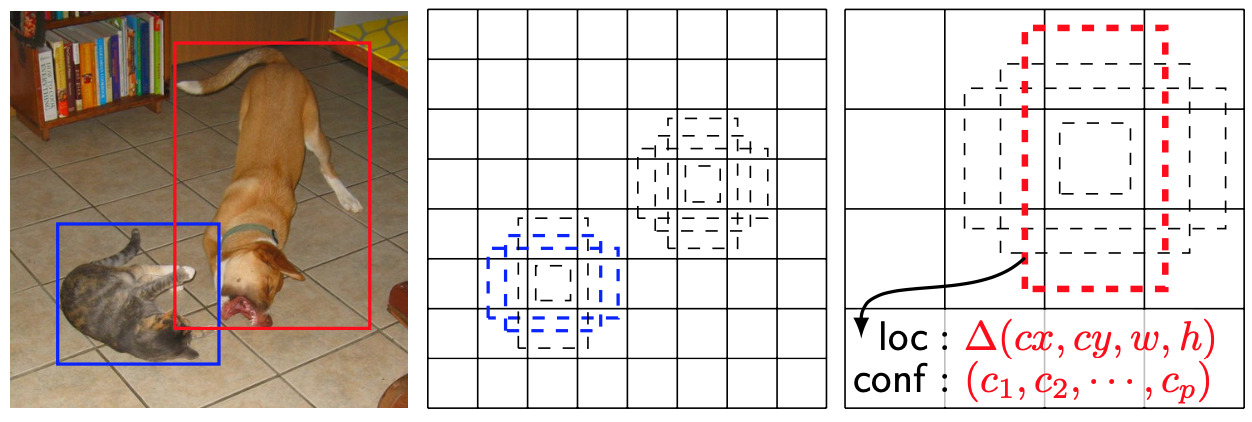
\includegraphics[width=11cm] {images/ssd_anchor}
        \caption{Cách đề xuất khu vực mỏ neo\index{khu vực mỏ neo} của mô hình SSD. (Nguồn: \cite{liu2016ssd})}
        \label{fig:ssd_anchor}
    \end{figure}
    
    \noindent
    SSD cũng sử dụng bản đồ đặc trưng\index{bản đồ đặc trưng} như là các dạng grid\index{grid} của ảnh đầu vào nhưng thay vì sử dụng một grid\index{grid} như YOLO thì SSD sử dụng nhiều grid\index{grid} từ nhiều bản đồ đặc trưng\index{bản đồ đặc trưng} có cách kích thước khác nhau.
    Với mỗi grid\index{grid} tạo bởi một bản đồ đặc trưng\index{bản đồ đặc trưng} có kích thước $m × n$, SSD trả đầu ra dự đoán có kích thước $m × n × (k × (c + 4))$.
    Nếu tâm của một hộp giới hạn\index{hộp giới hạn} nằm trong ô nào trên grid\index{grid}, ô đó sẽ cần phải được dự đoán là chứa đối tượng.
    Mỗi ô trên grid\index{grid} sẽ được mô hình dự đoán $(k × (c + 4))$ giá trị, trong đó: \\
    - k là số lượng hộp giới hạn\index{hộp giới hạn} dự đoán. \\
    - 4 là 4 giá trị x, y, w, h đại diện cho hộp giới hạn\index{hộp giới hạn} được dự đoán. \\
    - c là số lượng lớp đối tượng\index{lớp đối tượng} trong bài toán nhận diện đối tượng\index{nhận diện đối tượng}.
    Mỗi giá trị dự đoán trong c là giá trị xác suất khu vực mỏ neo\index{khu vực mỏ neo} đó là đối tượng nào.

    \noindent
    Với ý tưởng khởi tạo khu vực mỏ neo\index{khu vực mỏ neo} như trên, nhóm tác giả của RetinaNet\index{RetinaNet} đã chỉ ra một vấn đề nghiêm trọng mà các mô hình nhận diện đối tượng\index{nhận diện đối tượng} một pha\index{một pha} nói chung gặp phải đó là vấn đề mất cân bằng dữ liệu\index{mất cân bằng dữ liệu} trong quá trình huấn luyện mô hình.
    Cụ thể, vấn đề mất cân bằng ở đây xảy ra chủ yếu do sự chênh lệch giữa phần ảnh là foreground\index{foreground} và phần ảnh là background\index{background}, hay nói cách khác là phần ảnh chứa đối tượng và phần ảnh không chứa đối tượng. \\
    Các mô hình nhận diện đối tượng\index{nhận diện đối tượng} hai pha\index{hai pha} không thật sự gặp phải vấn đề mất cân bằng dữ liệu\index{mất cân bằng dữ liệu} này.

    \subsubsection*{Hàm mất mát Focal}
    Để giải quyết vấn đề mất cân bằng dữ liệu\index{mất cân bằng dữ liệu} nói trên, nhóm tác giả của RetinaNet\index{RetinaNet} đã đề xuất hàm mất mát Focus\index{mất mát Focus} dựa trên nền tảng của hàm mất mát entropy chéo nhị phân\index{hàm mất mát entropy chéo nhị phân} giải quyết vấn đề mất cân bằng dữ liệu\index{mất cân bằng dữ liệu} nghiêm trọng.
    Nhóm tác giả chú thích rằng hàm mất mát Focal\index{hàm mất mát Focal} hiệu quả đối với cả bài toán phân lớp với nhiều hơn hai lớp nhưng để đơn giản hoá, nhóm tác giả sử dụng hàm mất mát entropy chéo nhị phân\index{hàm mất mát entropy chéo nhị phân}.

    \begin{equation}
        \label{eq:bce}
        CE(p,y) = 
        \begin{cases}
            -\log(p) &\text{if $y = 1$} \\
            -\log (1 - p) &\text{otherwise.}
        \end{cases}
    \end{equation}

    \noindent
    trong đó: \\
    - y là giá trị groundtruth\index{groundtruth} (0 đối với khu vực mỏ neo\index{khu vực mỏ neo} không chứa đối tượng và 1 đối với khu vực mỏ neo\index{khu vực mỏ neo} chứa đối tượng). \\
    - p là giá trị xác suất mà mô hình dự đoán khu vực mỏ neo\index{khu vực mỏ neo} đó chứa đối tượng. \\
    Để ngắn gọn, nhóm tác giả quy ước lại như sau:

    \begin{equation}
        \label{eq:bce}
        p_\textrm{t} =
        \begin{cases}
            p &\text{if $y = 1$} \\
            1 - p &\text{otherwise,}
        \end{cases}
    \end{equation}

    \noindent
    từ đó, hàm mất mát entropy chéo\index{hàm mất mát entropy chéo} được viết lại thành

    \begin{equation}
        CE(p,y) = CE(p_\textrm{t}) = - \log (p_\textrm{t})
    \end{equation}

    \noindent
    Một cấu hình khác của hàm mất mát entropy chéo\index{hàm mất mát entropy chéo} là \textit{hàm mất mát entropy chéo cân bằng}\index{hàm mất mát entropy chéo cân bằng}, được sinh ra bằng việc đánh trọng số cho từng số hạng của hàm mất mát entropy chéo\index{hàm mất mát entropy chéo} ban đầu

    \begin{equation}
        CE(p,y) = - \alpha_\textrm{t} \log (p_\textrm{t})
    \end{equation}

    \noindent
    trong đó: \\
    - $\alpha_\textrm{t}$ là trọng số tương ứng với số hạng $p_\textrm{t}$.
    Trọng số $\alpha_\textrm{t}$ có thể được tính dựa trên tần suất xuất hiện của các lớp trong bộ dữ liệu hoặc là một hyperpameter.

    \noindent
    Hàm hàm mất mát entropy chéo cân bằng\index{hàm mất mát entropy chéo cân bằng} có thể đã giúp giảm bớt hiệu ứng mất cân bằng dữ liệu\index{mất cân bằng dữ liệu} lên trên giá trị hàm mất mát.
    Tuy nhiên, việc gán trọng số như hàm hàm mất mát entropy chéo cân bằng\index{hàm mất mát entropy chéo cân bằng} không phân biệt được giữa những mẫu dữ liệu dễ và khó.
    Nhóm tác giả, từ đó, đề xuất hàm \textit{mất mát Focus} không những giúp giải quyết vấn đề mất cân bằng dữ liệu\index{mất cân bằng dữ liệu} mà còn giúp mô hình tập trung vào những mẫu dữ liệu \textit{không chứa đối tượng} nhưng khó và dễ nhầm lẫn thành \textit{chứa đối tượng}.

    \begin{equation}
        FL(p_\textrm{t}) = - (1 - p_\textrm{t})^\gamma \log (p_\textrm{t})
    \end{equation}

    \noindent
    trong đó: \\
    - $(1 - p_\textrm{t})$ là thành phần đánh giá độ dễ hay khó của mẫu dữ liệu.
    Với những mẫu dễ và mô hình đã được huấn luyện tốt, giá trị $(1 - p_\textrm{t})$ sẽ nhỏ và những mẫu này sẽ gây ít ảnh hưởng trong quá trình huấn luyện mô hình. \\
    - $\gamma$ được nhóm tác giả gọi là \textit{focusing parameter}, dùng để xác định mức độ tập trung của mô hình lên các mẫu dữ liệu không chứa đối tượng.
    Với $\gamma = 0$, hàm FL lúc này tương tự với hàm CE.
    Trong các thí nghiệm của RetinaNet, giá trị $\gamma = 2$ là tốt nhất.

    \begin{figure}[H]
        \centering
        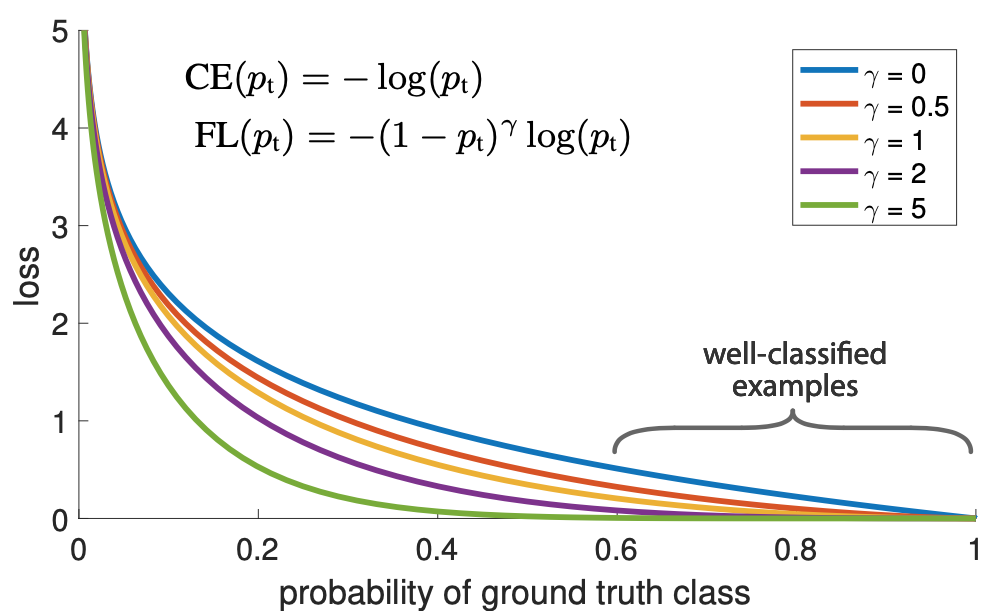
\includegraphics[width=8cm] {images/retinanet_focal_loss_curve}
        \caption{So sánh kết quả với các tham số của hàm mất mát Focal\index{hàm mất mát Focal} với hàm mất mát entropy chéo. (Nguồn: \cite{lin2017focal})}
        \label{fig:retinanet_focal_loss_curve}
    \end{figure}

    \noindent
    Ngoài ra, nhóm tác giả còn đề xuất một dạng khác của hàm FL bằng việc sử dụng thêm một tham số $\alpha$ và trong các thí nghiệm, dạng này cho kết quả tốt hơn một chút so với dạng hàm FL không sử dụng $\alpha$.

    \begin{equation}
        FL(p_\textrm{t}) = - \alpha_\textrm{t} (1 - p_\textrm{t})^\gamma \log (p_\textrm{t})
    \end{equation}
    
    \subsubsection*{Kiến trúc mô hình RetinaNet}
    RetinaNet\index{RetinaNet} gồm có các thành phần: \\
    - Phần \textit{mô hình xương sống FPN} được sử dụng nhằm trích xuất đặc trưng của ảnh đầu vào với nhiều kích thước đặc trưng khác nhau. \\
    - Phần trích xuất khu vực mỏ neo\index{khu vực mỏ neo} được thực hiện tương tự với cách trích xuất của mô hình RPN. \\
    Tuy nhiên, nhóm tác giả đã thử nghiệm và bổ sung thêm các kích thước $2^{0}$, $2^{1/3}$, $2^{2/3}$ của khu vực mỏ neo\index{khu vực mỏ neo} để đạt kết quả tốt hơn.
    Các khu vực mỏ neo\index{khu vực mỏ neo} được gán groundtruth\index{groundtruth} với chiến lược tương tự như trong Faster R-CNN\index{Faster R-CNN} \cite{ren2015faster} và (2) thay đổi threshold IoU\index{IoU} để gán nhãn cho từng khu vực mỏ neo\index{khu vực mỏ neo}.

    \begin{figure}[H]
        \centering
        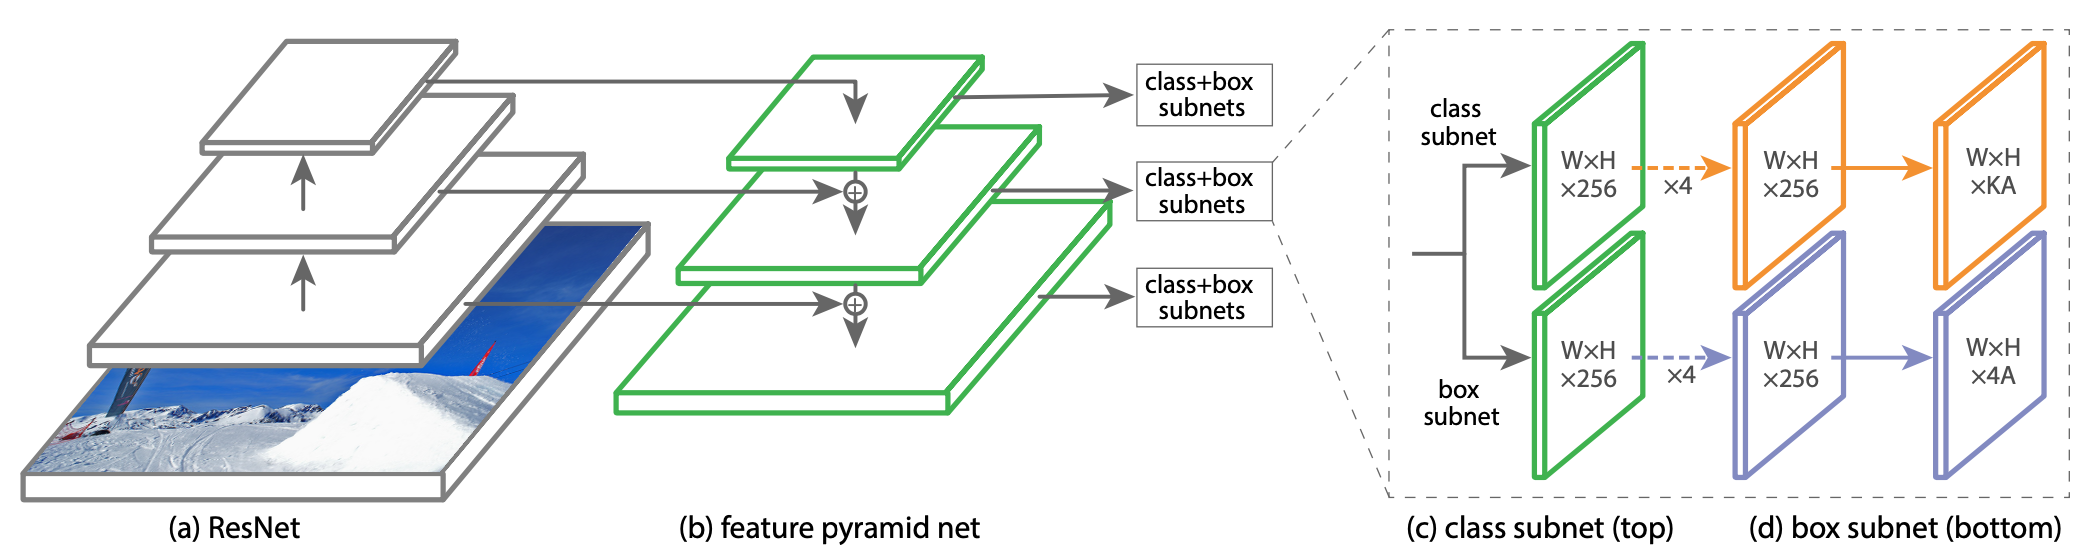
\includegraphics[width=14cm] {images/retinanet_model}
        \caption{Kiến trúc mô hình RetinaNet. (Nguồn: \cite{lin2017focal})}
        \label{fig:retinanet_model}
    \end{figure}

    \noindent
    - Phần \textit{Classification Subnet} được chia sẻ giữa tất cả các bản đồ đặc trưng\index{bản đồ đặc trưng} của mô hình xương sống FPN\index{FPN}, gồm các lớp Conv\index{lớp Conv} 3x3xC và lớp Conv\index{lớp Conv} cuối cùng 3x3xKA.
    Trong đó, K là số lượng lớp đối tượng\index{lớp đối tượng} trong bài toán nhận diện đối tượng\index{nhận diện đối tượng}, A là số lượng khu vực mỏ neo\index{khu vực mỏ neo} tại vị trí trên mỗi bản đồ đặc trưng\index{bản đồ đặc trưng} của mô hình xương sống FPN\index{FPN} (tác giả chọn $A = 9$), C là số lượng channel\index{channel} của lớp Conv\index{lớp Conv} (tác giả chọn $C = 256$). \\
    - Phần \textit{Box Regression Subnet} được thiết kế khác với cách thiết kế trong mô hình Faster R-CNN\index{Faster R-CNN} \cite{ren2015faster} khi không dùng chung các lớp Conv\index{lớp Conv} với \textit{Classification Subnet}.
    \textit{Box Regression Subnet} cũng gồm các lớp Conv\index{lớp Conv} 3x3xC và lớp Conv\index{lớp Conv} cuối cùng 3x3x4A.
    Trong đó, A là số lượng khu vực mỏ neo\index{khu vực mỏ neo} tại vị trí trên mỗi bản đồ đặc trưng\index{bản đồ đặc trưng}của mô hình xương sống FPN\index{FPN} (tác giả chọn $A = 9$), 4 là 4 độ lệch trong toạ độ của hộp giới hạn\index{hộp giới hạn} dự đoán so với groundtruth\index{groundtruth}, C là số lượng channel\index{channel} của lớp Conv\index{lớp Conv} (tác giả chọn $C = 256$).

    \subsubsection*{Kết luận về mô hình RetinaNet}
    Mô hình RetinaNet\index{RetinaNet} ra đời là một bước tiến lớn đối với việc giải quyết bài toán nhận diện đối tượng\index{nhận diện đối tượng} khi nó giải quyết vấn đề mất cân bằng dữ liệu\index{mất cân bằng dữ liệu} của các mô hình một pha\index{một pha} giúp tăng độ chính xác của mô hình ngang bằng với các mô hình hai pha\index{hai pha} nhưng vẫn duy trì được một tốc độ nhanh và có thể sử dụng trong thời gian thực. \\
    Mô hình RetinaNet\index{RetinaNet} cho đến nay vẫn là một mô hình tốt để giải quyết bài toán nhận diện đối tượng\index{nhận diện đối tượng}.
}